\documentclass[a4paper,12pt,numbers=noenddot]{scrreport}

\usepackage[german]{datetime2}
\usepackage[onehalfspacing]{setspace}
\usepackage[utf8]{inputenc}
\usepackage{amsmath, amsfonts, amssymb, amsthm}
\usepackage{multirow}
\usepackage{mathrsfs}
\usepackage{colortbl}
\usepackage{enumerate}
\usepackage{graphicx} % Required for inserting images

\usepackage{scrlayer-scrpage}
\renewcommand*{\chapterpagestyle}{scrheadings}
\clearpairofpagestyles

\ohead{\normalfont \today}
\chead{\normalfont Algebraic Automata Theory}
\ihead{\normalfont \rightmark}

\ofoot{\normalfont Seite~\pagemark}
\cfoot{\normalfont CAU Kiel - Technische Fakultät}
\ifoot{\normalfont Eric Hotho, Klaas Pelzer}

\KOMAoptions{headsepline=true,footsepline=true}
\renewcommand*{\chapterheadstartvskip}{\vspace*{-.4cm}}
\renewcommand*{\chapterheadendvskip}{\vspace{.5cm}}

\setlength{\parindent}{0pt}

\setkomafont{chapter}{\LARGE}
\setkomafont{section}{\Large}
\setkomafont{subsection}{\large}
\setkomafont{subsubsection}{\normalsize}
\setkomafont{paragraph}{\normalsize}
\setkomafont{subparagraph}{\small}
\usepackage[htt]{hyphenat}
\usepackage[german]{babel}
\setcounter{chapter}{9}

\def\lsk{\left<}
\def\rsk{\right>}
\DeclareMathOperator{\mmod}{mod}

\begin{document}
\automark{section}
\automark{chapter}

\chapter{}
\section{}
We prove that a connected transformation group $A=(Q,G)$ is primitive iff it is irreducable.

primiitive $\implies$ irreducable: $A$ does not contain any primitive block $P \subset Q$ with $|P| \geq 2$
and $P \cap Pg \in \{P, \emptyset \}$ for all $g \in G$.
Suppose $A$ is reducable which means $|Q| \leq 1$ or there exists an admissable partition of $Q$ that is not trivial.
Since $G$ is transitive, $Q$ has at least two states which contradicts $|Q| \leq 1$.\\
Suppose there exists a non trivial admissable partition $\pi = \{H_i\}_{i \in I}$.
For all $i \in I$ and all $g \in G$ there exists $j \in I$ with $H_ig \subseteq H_j$.
Notice, $i \neq j$ because otherwise $P = H_i$ and $P \cap Pg = P$.
Thus, $H_i \cap H_j = \emptyset$ but then it follows that $P \subseteq H_i$ and $P \cap Pg = \emptyset$ - a contradiction.

irreducable $\implies$ primitive: $A$ is irreducable which means $|Q| > 1$ and all admissable partitions are trivial.
Suppose $A$ is imprimitive.
Thus, the group produces a block system with primitive blocks $P \subset Q$ with $|P| \geq 2$ and $P \cap Pg \in \{P, \emptyset\}$ for all $g \in G$.

A primitive block produces a partition by the right coset  $\pi = \{Pg | g \in G\}$.
We prove that by showing $Pg_1 \cap Pg_2 = \emptyset$.
Suppose there exists an element $x \in Pg_1 \cap Pg_2$.
Then $x = p_1g_1 = p_2g_2$ and $p_1 = p_2g_2g^{-1}_1$. 
Therefore $p_1 \in P$ and also $p_1 \in Pg_2g^{-1}_1$ following 
\begin{align*}
    P &= Pg_2g^{-1}_1\\
    Pg_1 &= Pg_2
\end{align*}
shows that $pg_1$ and $pg_2$ are in the same primitive block.

By Lemma 8.12 any subgroup and its right coset builds also an admissable partition which is not trivial due to $2 \leq |P| < |Q|$.
This contradicts the assumption $A$ being irreducable.

We showed that both directions hold true which concludes the proof.
\qed

\section{}
We want to show the following: Let $G$ be a finite group, then TS$(SM(\mathcal{G})) = (G,\mathsf{G})$ with $\mathsf{G}= \{ [g]|g\in G\}$.\\
For this lets have a look at the definitions:
\begin{align*}
    TS(SM(\mathcal{G})) &= TS((G,G,\delta)) \tag{Def. 8.10} \\
                        &= (G, S(\mathcal{G})) \tag{3.18} \\
                        &= (G, \mathsf{G}) \tag{(1), 3.10}\\ 
\end{align*}
Regarding (1), as per definition in the script $S(M) = \Sigma^+ \backslash \sim_M$ which describes the equivalence classes over all words of M defined by the congruence relation $\sim_M$, thus, it is equivalent to $\mathsf{G}= \{ [g]|g\in G\}$.
\qed
\section{}
\section{}
We begin by constructing the permutation machine as depicted in \ref{fig:permutation machine}.
\begin{figure}[h]
    \centering
    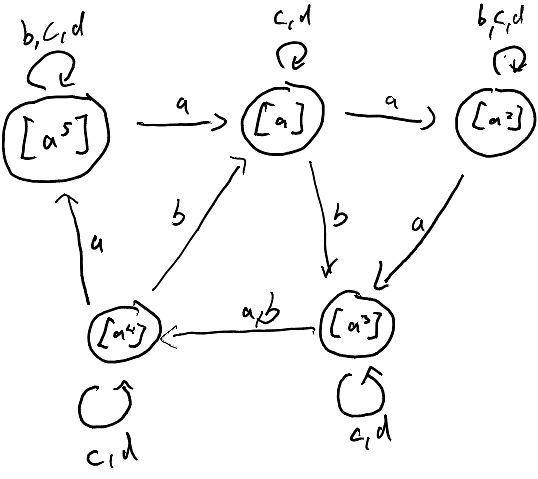
\includegraphics[width=0.5\linewidth]{Permutation_Machine.png}
    \caption{Permutation machine}
    \label{fig:permutation machine}
\end{figure}
Next we define the reset machine as follows: $N = (Q, (\mathbb{Z}_5 \times \Sigma) \cup \{\lambda\}, \delta')$ with \\
\begin{center}
    \begin{tabular}{ c | c c c c c }
        ~               & $q_0$         & $q_1$       & $q_2$       & $q_3$       & $q_4$\\
        \hline
        $\lambda$         & $q_0$         & $q_1$       & $q_2$       & $q_3$       & $q_4$ \\
        $([a], a)$      & $q_1$         & $q_2$       & $q_3$       & $q_4$       & $q_0$ \\
        $([a], c)$      & $\bot$        & $q_0$       & $\bot$      & $q_0$       & $q_0$ \\
        $([a], d)$      & $\bot$        & $\bot$      & $q_3$       & $q_3$       & $\bot$ \\
        $([a], b)$      & $q_2$          & $q_1$        & $q_3$        & $q_0$          & $q_4$ \\
        $([a^2], a)$    & $q_1$        & $q_2$        & $q_3$        & $q_4$        & $q_0$ \\
        $([a^2], c)$    & $q_4$        & $\bot$        & $q_4$        & $q_4$        & $\bot$ \\
        $([a^2], d)$    & $\bot$        & $q_2$        & $q_2$        & $\bot$        & $\bot$ \\
        $([a^2], b)$      & $q_0$          & $q_2$        & $q_4$        & $q_3$          & $q_1$ \\
        $([a^3], a)$    & $q_1$        & $q_2$        & $q_3$        & $q_4$        & $q_0$ \\
        $([a^3], c)$    & $\bot$        & $q_3$        & $q_3$        & $\bot$        & $q_3$ \\
        $([a^3], d)$    & $q_1$        & $q_1$        & $\bot$        & $\bot$        & $\bot$ \\
        $([a^3], b)$      & $q_1$          & $q_3$        & $q_2$        & $q_0$          & $q_4$ \\
        $([a^4], a)$    & $q_1$        & $q_2$            & $q_3$          & $q_4$      & $q_0$ \\
        $([a^4], c)$    & $q_2$        & $q_2$            & $\bot$          & $q_2$      & $\bot$ \\
        $([a^4], d)$    & $q_0$        & $\bot$           & $\bot$          & $\bot$      & $q_0$ \\
        $([a^4], b)$      & $q_2$          & $q_1$        & $q_4$        & $q_3$          & $q_0$ \\
        $([a^5], a)$    & $q_1$        & $q_2$            & $q_3$          & $q_4$      & $q_0$ \\
        $([a^5], c)$    & $q_1$        & $\bot$            & $q_1$          & $\bot$     & $q_1$ \\
        $([a^5], d)$    & $\bot$        & $\bot$           & $\bot$         & $q_4$      & $q_4$ \\
        $([a^5], b)$      & $q_0$          & $q_3$        & $q_2$        & $q_4$          & $q_1$ \\
    \end{tabular}
\end{center}
Then we get $TS(M) \leq N\omega P $.
\qed
\end{document}

